\chapter{Implementierung und Benchmarks}
Was wurde Implementiert und warum?
Die verwendete Bibliothek wurde in der Vorlesung High Performance Computing 1 entwickelt \cite{HPC1}.

Die Bibliothek ist in C++ geschrieben. Es sind Klassen für Matrizen und Vektoren implementiert, sowie einige BLAS-Routinen.

Die Matrix-Klassen erlauben den zugriff auf Matrixblöcke. 
Der folgender Code
\begin{lstlisting}
GenerelMatrix<T> A(5,5);
print(A);
print(A.block(2,2));
print(A.block(2,2).view(Trans::view));
\end{lstlisting}
erzeugt die Ausgabe
\begin{lstlisting} 
A = 
     0.4162   0.1087   0.6753  -0.3967  -0.5583
    -0.6969   0.4358   0.6349  -0.6566   0.8933
     0.9340   0.7451  -0.2149  -0.0740  -0.1027
     0.5809   0.5491   0.0163   0.1676  -0.9108
    -0.4325  -0.0732  -0.1847  -0.1897  -0.0717

A = 
    -0.2149  -0.0740  -0.1027
     0.0163   0.1676  -0.9108
    -0.1847  -0.1897  -0.0717

A = 
    -0.2149   0.0163  -0.1847
    -0.0740   0.1676  -0.1897
    -0.1027  -0.9108  -0.0717
\end{lstlisting}



Beispiel Ungeblockte QR Implementierung vom Algorithmus \ref{alg:unblockedqr}
\begin{lstlisting}
size_t mn = std::min(m,n);
DenseVector<T> work(mn);
for (std::size_t i = 0; i < mn; ++i){
  householderVector(A(i,i), A.col(i+1,i),tau(i));
  if (i < n && tau(i) != 0) {
    AII = A(i,i);
    A(i,i) = 1;
    mv(1, A.block(i,i+1).view(hpc::matvec::Trans::view),
       A.col(i,i), 0, work.block(i+1));
    rank1(-tau(i), A.col(i,i), work.block(i+1), 
          A.block(i,i+1));
    A(i,i) = AII;
  }
}
\end{lstlisting}

Die anderen Algorithem wurden analog Implementiert siehe Anhang.


\section{Aufwand}

Die QR-Zerlegung einer Matrix $A \in \mathbb{R}^{m \times n}$  erfordert
\begin{align*}
	n^2(m-\frac{1}{3} n) + {\cal O}(mn)
\end{align*}
Rechenoperationen. Quelle???

\subsection{FLOPS}
FLPOS (Floating Point Operations Per Second) 

\section{Fehlerschätzer}

Um zu testen ob die QR-Zerlegung korrekt ist, ist ein Fehlerschätzer notwendig.
Es wurde der Fehlerschätzer von ATLAS\cite{atlas} verwendet.
\begin{align}
	err = \dfrac{\|A - QR\|_i}{\|A\|_i \cdot \min(m,n) \cdot \varepsilon}
\end{align}
$\|\cdot\|_i$ ist eine passende Norm.
Die Matrizen $Q$ und $R$ sind die QR-Zerlegung der Matrix $A \in \mathbb{R}^{m \times n}$.
$\varepsilon$ ist die kleinste darstellbare Zahl.\\
Die QR-Zerlegung ist gut genug falls der Fehler kleiner 1 ist $ err < 1 $.

Als Norm wurde die Zeilensummennorm $\|\cdot\|_\infty$ gewählt.
Diese ist für eine Matrix $A \in \mathbb{R}^{m\times n}$ gegeben durch
\begin{align*}
	\|A\|_\infty = \max_{i=1,...,m} \sum_{j=1}^{n} |a_{ij}|
\end{align*}

Diese Norm wurde gewählt das sie sich leicht berechnen lässt.

$\epsilon$ ist auf dem Test-System $2.220446\cdot10^{-16}$


\section{Benchmarks}

\subsection{Test System}

Getestet wurde auf einem System mit einer Intel(R) Core(TM) i5-3470 CPU mit 3.20GHz. 

Die Theoretische peak performance errechnet sich aus der Taktrate mal die Registerbreite mal 2. Quelle???


Die CPU des Test Systems hat eine Taktrate von 3.20GHz.
Die AVX-Register sind 256-Bit groß. Darin haben 4 double Platz.

\begin{align*}
	\text{Taktrate} \cdot \text{Registerbreite} \cdot 2= 3,20 \text{ GHz} \cdot 4 \cdot 2 = 25,6 \text{ GFLOPs}
\end{align*}

\begin{figure}[H]
	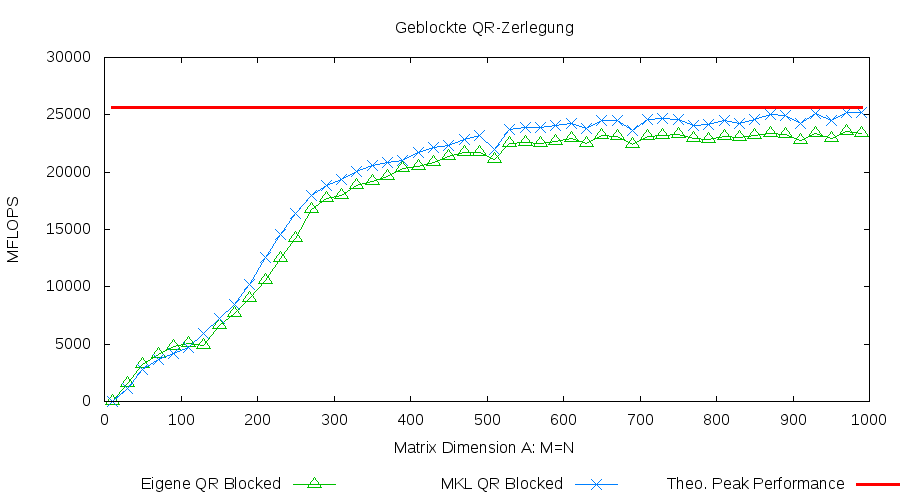
\includegraphics[width=\textwidth]{images/blk.png}
	\caption{Benchmark geblockte QR-Zerlegung}
	\label{img:blk}
\end{figure}

\begin{figure}[H]
	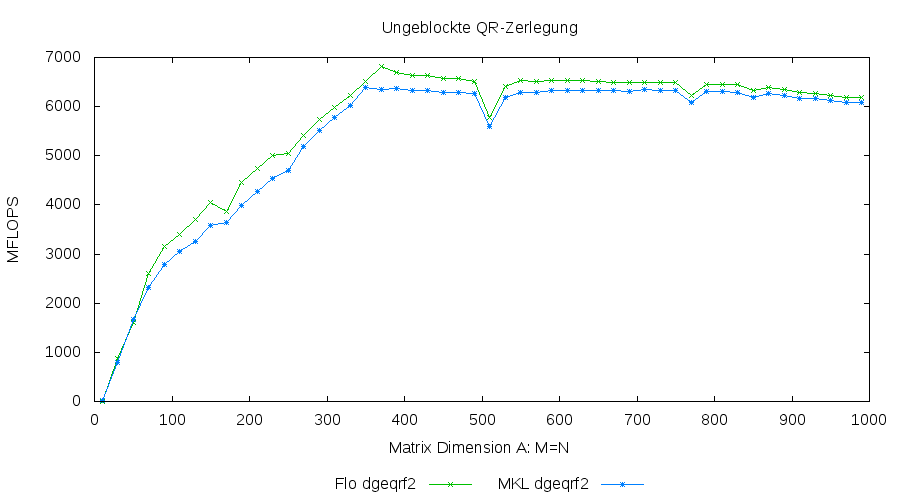
\includegraphics[width=\textwidth]{images/unblk.png}
	\caption{Benchmark ungeblockte QR-Zerlegung}
	\label{img:unblk}
\end{figure}

Dreiecke und Sternchen









	 
